\chapter{Les fonctionnalités CaWaQS-Viz}
\label{chap-features}

\renewcommand{\headrulewidth}{0.3pt}
\fancyhead[LE]{\thepage} \fancyhead[RE]{\nouppercase{\textbf{\leftmark}}}
\fancyhead[RO]{\thepage} \fancyhead[LO]{\nouppercase{\textbf{\rightmark}}}
\fancyfoot[L,C,R]{}

\setlength{\parindent}{0.35cm}

\minitoc
\newpage
\

\newpage

% ================================================================
\alertwarning{Toutes les sorties shapefile générés par \cwv sont temporaires. Si elles ne sont pas sauvegardées, elles ne seront plus accécibles à la réouverture du projet.}

\section{\gui{Calibration Tools}: Les outils de calibration}
\label{sec-calib-tools}

La boîte de dialogue \gui{Calibration Tools} (\cref{fig_DialogCalibrationTools})
permet d'accéder aux outils de calibration du modèle \cawaqs. Ces fonctionnalités
sont les suivantes :
\begin{itemize}
    \item un outil de modification des fichiers de paramétrisation des différents
        compartiments modélisés : \gui{Modify a parametrisation file} (\cref{sec-feat-modify-param})
        ;

    \item un outil de calcul des critères de performance de calibration du modèle
        : \gui{Statistical Criteria} (\cref{sec-critstat}) ;

    \item un outil de calcul du coefficient de ruissellement simulés : \gui{Run-off coefficient calculation}
        (\cref{sec-runoff-coef}) ;

    \item un outil de visualisation des chronique simulées et observée : \gui{Compare sim/obs}
        (\cref{sec-com-simobs}).
\end{itemize}

\begin{figure}[H]
    \centering
    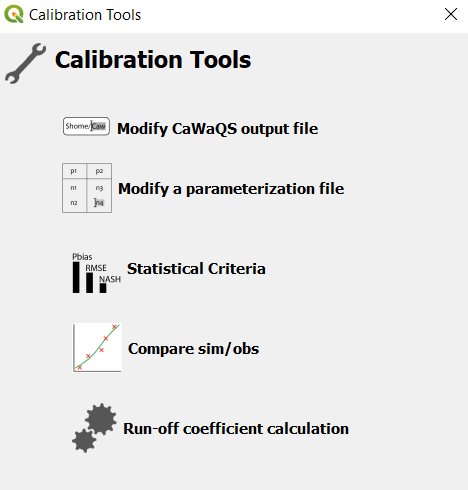
\includegraphics[width=0.65\linewidth]{
        2_application_user_guide/fig/DialogCalibrationTools.png
    }
    \caption{Boîte de dialogue des outils de calibration.}
    \label{fig_DialogCalibrationTools}
\end{figure}

\subsection{Modification des fichiers de paramétrisation}
\label{sec-feat-modify-param}

La modification des fichiers de paramétrisation peut être effectuée depuis la
boite de dialogue \gui{Modifying a parametrization file} (\cref{fig-dialog_modif_param_file}).
La résolution dépendra du fichier de calibration qui devra être sélectionné
dans le menu déroulant. L'affichage de la table se fera en cliquant sur

\includegraphics[height=0.45cm]{2_application_user_guide/fig/show.png}
. \\

Si la table attributaire affichée ne contient pas les champs du fichier de paramétrisation,
la résolution peut être liée à son fichier de paramétrisation dans la boite de
dialogue \gui{Lier la résolution à son fichier de paramétrisation} accessible en
cliquant sur
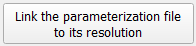
\includegraphics[height=0.55cm]{
    2_application_user_guide/fig/AccesDialogLinkParamResolution.png
}
.L'utilisation de cette boite de dialogue est décrite en \cref{sec-link_table}.

\begin{figure}[H]
    \centering
    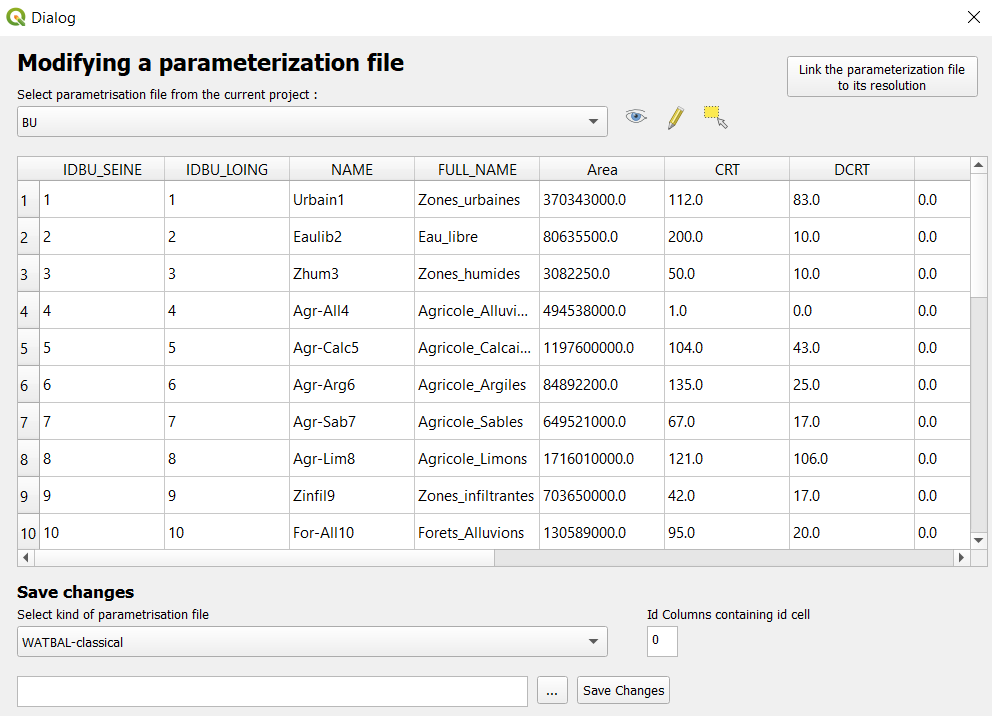
\includegraphics[width=1\linewidth]{
        2_application_user_guide/fig/DialogModifParamFile.png
    }
    \caption{Boîte de dialogue pour la modification des fichiers de
    paramétrisation.}
    \label{fig-dialog_modif_param_file}
\end{figure}

Une fois les paramètres modifiés dans la table affichée, elle peut être
enregistrée. Le nouveau chemin du fichier peut être renseigner en sélectionnant
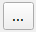
\includegraphics[height=0.45cm]{2_application_user_guide/fig/SelectPath.png}
. Renseigner l'identifiant de la colonne contenant l'identifiant ou le nom de la
cellule \footnote{ATTENTION : Pour rappel, les identifiants des colonnes débutent
à \textbf{0}.}.

\subsection{Lier une table attributaire à sa résolution}
\label{sec-link_table}

Les paramètres du fichier de paramétrisation seront directement importés en tant
que champ de la table attributaire du fichier de la résolution concernée. Pour créer
ce lien, un type de fichier de paramétrisation doit être choisi (en fonction du compartiment
et du type de fichier de paramétrisation), la résolution \cawaqs~ainsi que le chemin
d'accès à ce fichier de paramétrisation. Différents types de fichier de
paramétrisation existent et sont répertoriés dans le tableau
\ref{tab-type_param_file}.

\begin{figure}
    \centering
    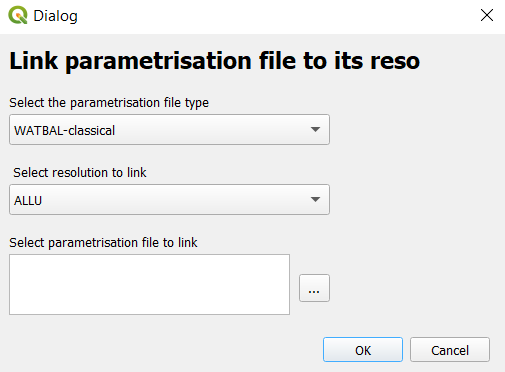
\includegraphics[width=0.7\linewidth]{
        2_application_user_guide/fig/DialogLinkTable.png
    }
    \caption{Boîte de dialogue permettant de lier une table attributaire à sa
    résolution.}
    \label{fig:enter-label}
\end{figure}

\begin{table}[H]
    \centering
    \begin{tabular}{m{4cm}|m{4cm}|m{4cm}}
        \hline
        \textbf{Compartiment} & \textbf{Type de fichier de paramétrisation} & \textbf{Paramètres renseignés dans la table}             \\
        \hline
        \script{WATBAL}       & Classical                                   & CRT, DCRT, R, FN, CQR, CQRMAX, CQI, CQIMAX et RNAP       \\
        \hline
        \script{WATBAL}       & Infiltration Excess                         & CRT, DCRT, R, FN, CQR, CQRMAX, CQI, CQIMAX, RNAP et RINF \\
        \hline
        \script{AQ}           & Transmissivity                              & T                                                        \\
        \hline
        \script{AQ}           & Storage (coefficient d'emmagasinement)      & S                                                        \\
        \hline
        \script{AQ}           & Conductance                                 & C                                                        \\
        \hline
        % Ajoutez plus de lignes de données si nécessaire
    \end{tabular}
    \caption{Les fichiers de paramétrisation pris en charge par \texttt{\cwv}.}
    \label{tab-type_param_file}
\end{table}

\subsection{\script{Statistical Criteria}: Calcul des critères statistiques de
performance au droit des points d'observation : }
\label{sec-critstat}

La boîte de dialogue \gui{Statistical Criteria} (\cref{fig-dialogstatisticalcriteria})
retourne une couche SIG suivant les géométries de la résolution d'observation
inhérente à la variable analysée. Chaque champ correspond à un critère statistique
donné. Les critères statistiques sélectionnés sont calculés sur la période
renseignée dans la partie \gui{Period for calculating statistical criteria}. \\

\subsubsection{Les critères statistiques calculé par la boite de dialogue \gui{Statistical criteria}}

\textbf{\gui{Pbias} : Bias [$\%$]}
\begin{equation*}
PBIAS = \frac{\sum(\hat{y}_i -y_i)}{\sum y_i} . 100
\quad \quad
\begin{array}{rl}
      
      y_i & : \text{variable simulée au temps $i$}\\
      O_i & : \text{variable observée au temps $i$}\\
\end{array}  
\end{equation*}

\textbf{\gui{Average SIM/OBS}}
\begin{equation*}
    A = \overline{\hat{y}} - \overline{y}
    \quad\quad
    \begin{array}{cc}
         \overline{\hat{y}} :& \text{moyenne des variables simulées} \\
         \overline{y} : & \text{moyenne des variables observées}
    \end{array}
\end{equation*}

\textbf{\gui{Nash} : Nash-Sutcliffe Model Efficiency} \citep{nash1970}
\begin{equation*}
    NSE = 1 - \frac{\sum_{i=1}^n (y_i - \hat{y}_i)^2}{\sum_{i=1}^n (y_i - \overline{y})^2}
    \quad \quad 
    \begin{array}{ll}
         y_i :& \text{variable réelle au temps } i \\
        \hat{y}_i :& \text{variable prédite au temps } i \\
    \end{array}
\end{equation*}

\textbf{\gui{RMSE} - Root Mean Squared Error} 
\begin{equation*}
RMSE = \sqrt{\frac{1}{n} \sum_{i=1}^{n} (y_i - \hat{y}_i)^2}
\quad \text{où} \quad
\begin{array}{ll}
    n :& \text{Nombre total jour de simulation} \\
    y_i :& \text{variable réelle au temps } i \\
    \hat{y}_i :& \text{variable prédite au temps } i \\
\end{array}
\end{equation*}

\textbf{\gui{KGE} - Kling-Gupta Efficiency} \citep{gupta2012}
\begin{equation}
    KGE = 1 - \sqrt{(r - 1)^2 + (\alpha - 1)^2 + (\beta - 1)^2} 
    \quad \quad
    \begin{array}{ll}
         r & : \text{coefficient de corrélation de Pearson} \\ 
         & \text{entre les série de variables simulées} \\ 
         & \text{et observées} \\
        \alpha & : \text{rapport des écarts-types simulés et observés} \\
        \beta  & : \text{biais moyen entre les séries simulées et observées}
    \end{array}
\end{equation}





Les critères suivants sont calculés automatiquement : $\overline{y}$, $\overline{\hat{y}}$, $\frac{\overline{\hat{y}}}{\overline{y}}$, $\sigma y$,  $\sigma \hat{y}$, $\frac{\sigma \hat{y}}{\sigma y}$.

\subsubsection{Sortie de la boite de dialogue \gui{Statistical Criteria}}
\label{sec_stats_crits}

La boite de dialogue génère les critères statistiques : 
\begin{itemize}
    \item aux droits des points d'observation,  
    \item à l'échelle de la couche aquifère dans le cas de simulation avec un compartiment aquifère ;
    \item à l'échelle de l'hydrosystème dans le cas de simulation avec un compartiment aquifère.
\end{itemize}
\vspace{0.3cm}

\underline{\textbf{Critères statistiques calculés aux droits des points d'observation}}\\
La boite de dialogue génère la table des critères statistiques au droit des points d'observation sous le format \script{shapefile} et \script{texte}. Le fichier Shapefile est introduit directement dans le projet \script{QGIS} courant, tandis que le fichier texte se trouvera dans le répertoire \script{../PostProcessing/STATS\_CRITS}. 
Les critères de sortie sont contenus dans les champs de chaque point de mesure sous les appels définis dans la table \ref{tab_statistical_criteria_crits_fields}.

\vspace{0.2cm}
\underline{\textbf{Critères statistiques calculés à l'échelle des unités aquifères}}\\
Dans le cas d'un calcul des critères statistiques sur le compartiment aquifère, un fichier \script{texte} enregistré dans le répertoire de \gui{Post-Processing} sous \script{../PostProcessing/STATS\_CRITS/AQ\_crits\_xxxx\_xxxx.txt}. Ce fichier recense les critères statistiques listés dans la table \ref{tab_statistical_criteria_crits_fields} défini à l'échelle de chaque unité aquifère. 

\vspace{0.2cm}
\underline{\textbf{Critère statiques calculés à l'échelle de l'hydrosystème}} \\
Les critère statistiques sont définis à l'échelle de l'hydrosystème sur la charge hydraulique en nappe. Ces critères écrits dans le fichiers \script{../PostProcessing/STATS\_CRITS/AQ\_crits\_xxxx\_xxxx.txt}. \\


\begin{table}[H]
    \centering
    \renewcommand{\arraystretch}{1.2}
    \resizebox{\textwidth}{!}{
        \begin{tabular}{rl}
        \hline
        \textbf{Nom du champ de la table de sortie} &  \textbf{Critère statistique} \\
        \hline
        \gui{NObs} & Nombre d'observations sur la période sélectionnée \\
        \gui{AObs} & Moyenne des variables observées \\
        \gui{ASIM} & Moyenne des variables simulées \\ 
        \gui{SUM\_RATIO} & Ratio de la somme des variables simulées et de la somme des variables observées \\
        \gui{StdObs} & Ecart-type des variables observées \\ 
        \gui{StdSim} & Ecart-type des variable simulées \\
        \gui{STD\_RATION} & Ratio des écart-types des variables observées et simulées \\
        \gui{PBAIS} & Biais  [\%] \\
        \gui{AVERAGE\ SIM/OBS} & Ratio moyen entre les variables simulées et observées \\
        \gui{KGE} & Kling-Gupta Efficiency \\
        \gui{NASH} & Nash-Sutcliffe Model Efficiency \\ 
        \gui{RMSE} & Root Mean Squared Error \\
        \hline
        \end{tabular}
    }
    \caption{Nom des champs des tables de sorties pour chaque critère statistique}
    \label{tab_statistical_criteria_crits_fields}
\end{table}


\begin{figure}[H]
    \centering
    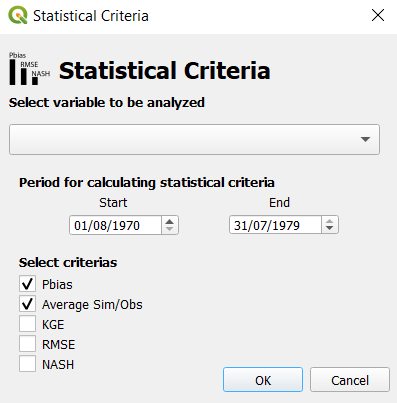
\includegraphics[width=0.5\linewidth]{
        2_application_user_guide/fig/DialogStatisticalCriteria.png
    }
    \caption{Boîte de dialogue \gui{Statistical Criteria}.}
    \label{fig-dialogstatisticalcriteria}
\end{figure}


\subsection{\script{Run-off coefficient calculation}: Calcul du coefficient de
ruissellement au droit des stations de mesure de débit}
\label{sec-runoff-coef}

Cette boîte de dialogue permet de calculer le coefficient de ruissellement simulé
et observé au droit des stations de mesures de débit. \\

\begin{figure}[H]
    \centering
    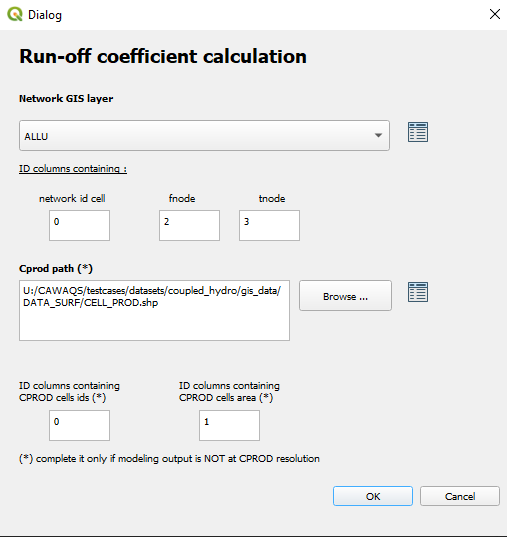
\includegraphics[width=0.5\linewidth]{
        2_application_user_guide/fig/DialogRunOffCalclulation.png
    }
    \caption{Boîte de dialogue pour le calcul du coefficient de ruissellement.}
    \label{fig-DialogRunoffCoeff}
\end{figure}

Cette boîte prend en paramètres la résolution du schéma hydrologique de surface
à l'échelle des tronçons rivières et de la résolution de surface \cawaqs~des
cellules de production (bassins versants unitaires ou \script{Cprod}). Pour la
première, le numéro de la colonne contenant les identifiants de tronçon, des
\script{Fnode} et \script{Tnode} sera à renseigner. Pour la seconde, l'identifiant
des champs contenant l'identifiant des cellules de production, d'une part, et
des surfaces de cellules. \\

Si la résolution de surface définie dans la configuration \cwv~est déjà celle
des cellules de production, dans ce cas, il ne sera pas nécessaire de renseigner
ici la partie inférieure de la boite de dialogue.

Deux nouvelles résolutions (\textit{shapefiles}) seront retournées par la boite de
dialogue et ajoutées au projet SIG courant :
\begin{itemize}
    \item \gui{CATCH} qui contient les bassin drainés par chaque station de
        mesure ;

    \item \gui{CATCH\_SURF}, produit de l'intersection entre la résolution de surface
        défini dans la configuration de \cwv~et de \gui{CATCH}. Sa table attributaire
        contient plusieurs champs :
        \begin{itemize}
            \item[$-$] \gui{CATCH\_ID} et \gui{CATCH\_SURF}: l'identifiant du
                bassin versant drainé par la station et sa surface ;

            \item[$-$] \gui{ID\_OBS} : l'identifiant la station de mesure ;

            \item[$-$] \gui{SURF\_ID} : la surface de la cellule de surface
                issue de la résolution de surface définie dans la configuration
                \cwv~;

            \item[$-$] \gui{SURF\_SURF} : sa surface ;

            \item[$-$] \gui{INTER\_ID} : l'identifiant de la cellule d'intersection
                ;

            \item[$-$] \gui{INTER\_SURF} : la surface d'intersection.
        \end{itemize}
\end{itemize}

Ces résolutions sont enregistrées au format temporaire. Il est laissé libre à l'utilisateur
de les enregistrer pour une future réutilisation. Si \cwv~reconnaît ces
résolutions dans le projet QGIS courant, elles seront réutilisées pour le calcul
des coefficients de ruissellement. \\

Ces coefficients peuvent être retrouvés dans la table attributaire de la couche d'observation
de débit renseignée à l'étape de configuration. Deux nouveaux champs sont alors
ajoutés : \gui{QruissSim} et \gui{QruissObs} désigant respectivement le
coefficient de ruissellement simulé par \cawaqs~et celui observé au droit des
stations de mesure.

\section{\script{Compare sim/obs}: Comparaison des chroniques observées et
simulées}
\label{sec-com-simobs}

Ce module de calcul permet la comparaison entre les simulations et les observations renseignées au travers de plusieurs types de rendu : 
\begin{itemize}
    \item en cliquant sur \gui{PDF printout}, un fichier \script{pdf} est généré. Les chroniques simulées et observées sont présentées avec les critères statistiques référencés dans le tableau \ref{tab_statistical_criteria_crits_fields} ;
    \item en cliquant sur \gui{Interactiv graphics}, un format \script{html} reprend le format de présentation des chroniques du format \script{pdf} de manière interactive dans le navigateur par défaut ;
    \item en cliquant sur \gui{Statistical criteria}, la boite de dialog \gui{Statistical Criteria} (\ref{sec-critstat}) s'ouvre. Les paramètres renseignés de la boite de dialogue \gui{Compare Sim-Obs} (dates, compartiement et unité de mesure des observation) sont reportés dans la boite de dialogue \gui{Statistical Criteria}. 
\end{itemize}

\begin{figure}[H]
    \centering
    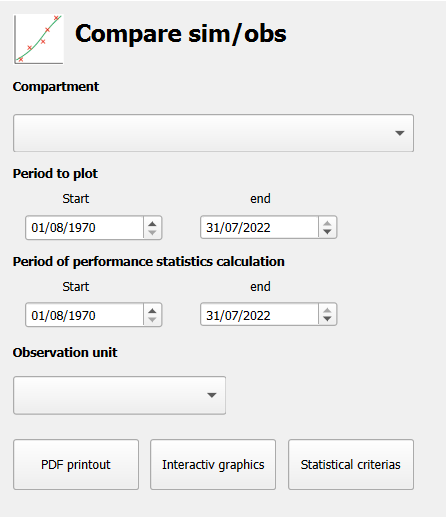
\includegraphics[width=0.45\linewidth]{
        2_application_user_guide/fig/DialogCompareSimObs.png
    }
    \caption{Fenêtre de dialogue \gui{Compare sim/obs}.}
    \label{fig-dialogCompareSimObs}
\end{figure}

Le type de compartiment (\script{AQ} = aquifère et \script{HYD} = réseau
hydrographique) est à sélectionner dans la liste déroulante située dans la partie
supérieure de la boite de dialogue (\cref{fig-dialogCompareSimObs}). Les
périodes d'impression des séries temporelles ainsi que celles du calcul des
critères statistiques sont également à renseigner. L'unité des observations de débit, utilisée pour l'exploitation des simulations du compartiment \gui{HYD} est à préciser dans le menu déroulant \gui{Observation unit}. Elle est optionnelle pour l'exploitation du compartiment \gui{AQ}. \\

Un message d'information sera affiché dans l'interface QGIS à la fin de l'exécution
de cette tâche et pointera le répertoire de post-traitement. Les fichiers
\script{.pdf} issus de l'analyse du compartiment \script{HYD} seront nommés par
défaut \gui{SIM\_OBS\_HYD.pdf}. Ceux issus de l'analyse du compartiment aquifère
seront nommés \gui{SIM\_OBS\_AQ.pdf}. Chaque page de ce document correspond à
une station de mesure.

\section{\script{Spatial Map}: Cartographie spatiale des variables hydrologiques}
\label{sec-spatial-map}

Cet outil spatialise le bilan hydrique de surface sous format \script{.shp}. Le bilan peut être produit à une fréquence annuelle, mensuelle ou journalière (à renseigner dans le champ \script{frequence}). L'agrégation temporelle peut être réalisée par une moyenne, une somme, un maximum ou un minimum (à renseigner dans le champ \script{agregator}).


\begin{figure}[H]
    \centering
    \begin{subfigure}
        [b]{0.48\linewidth}
        \centering
        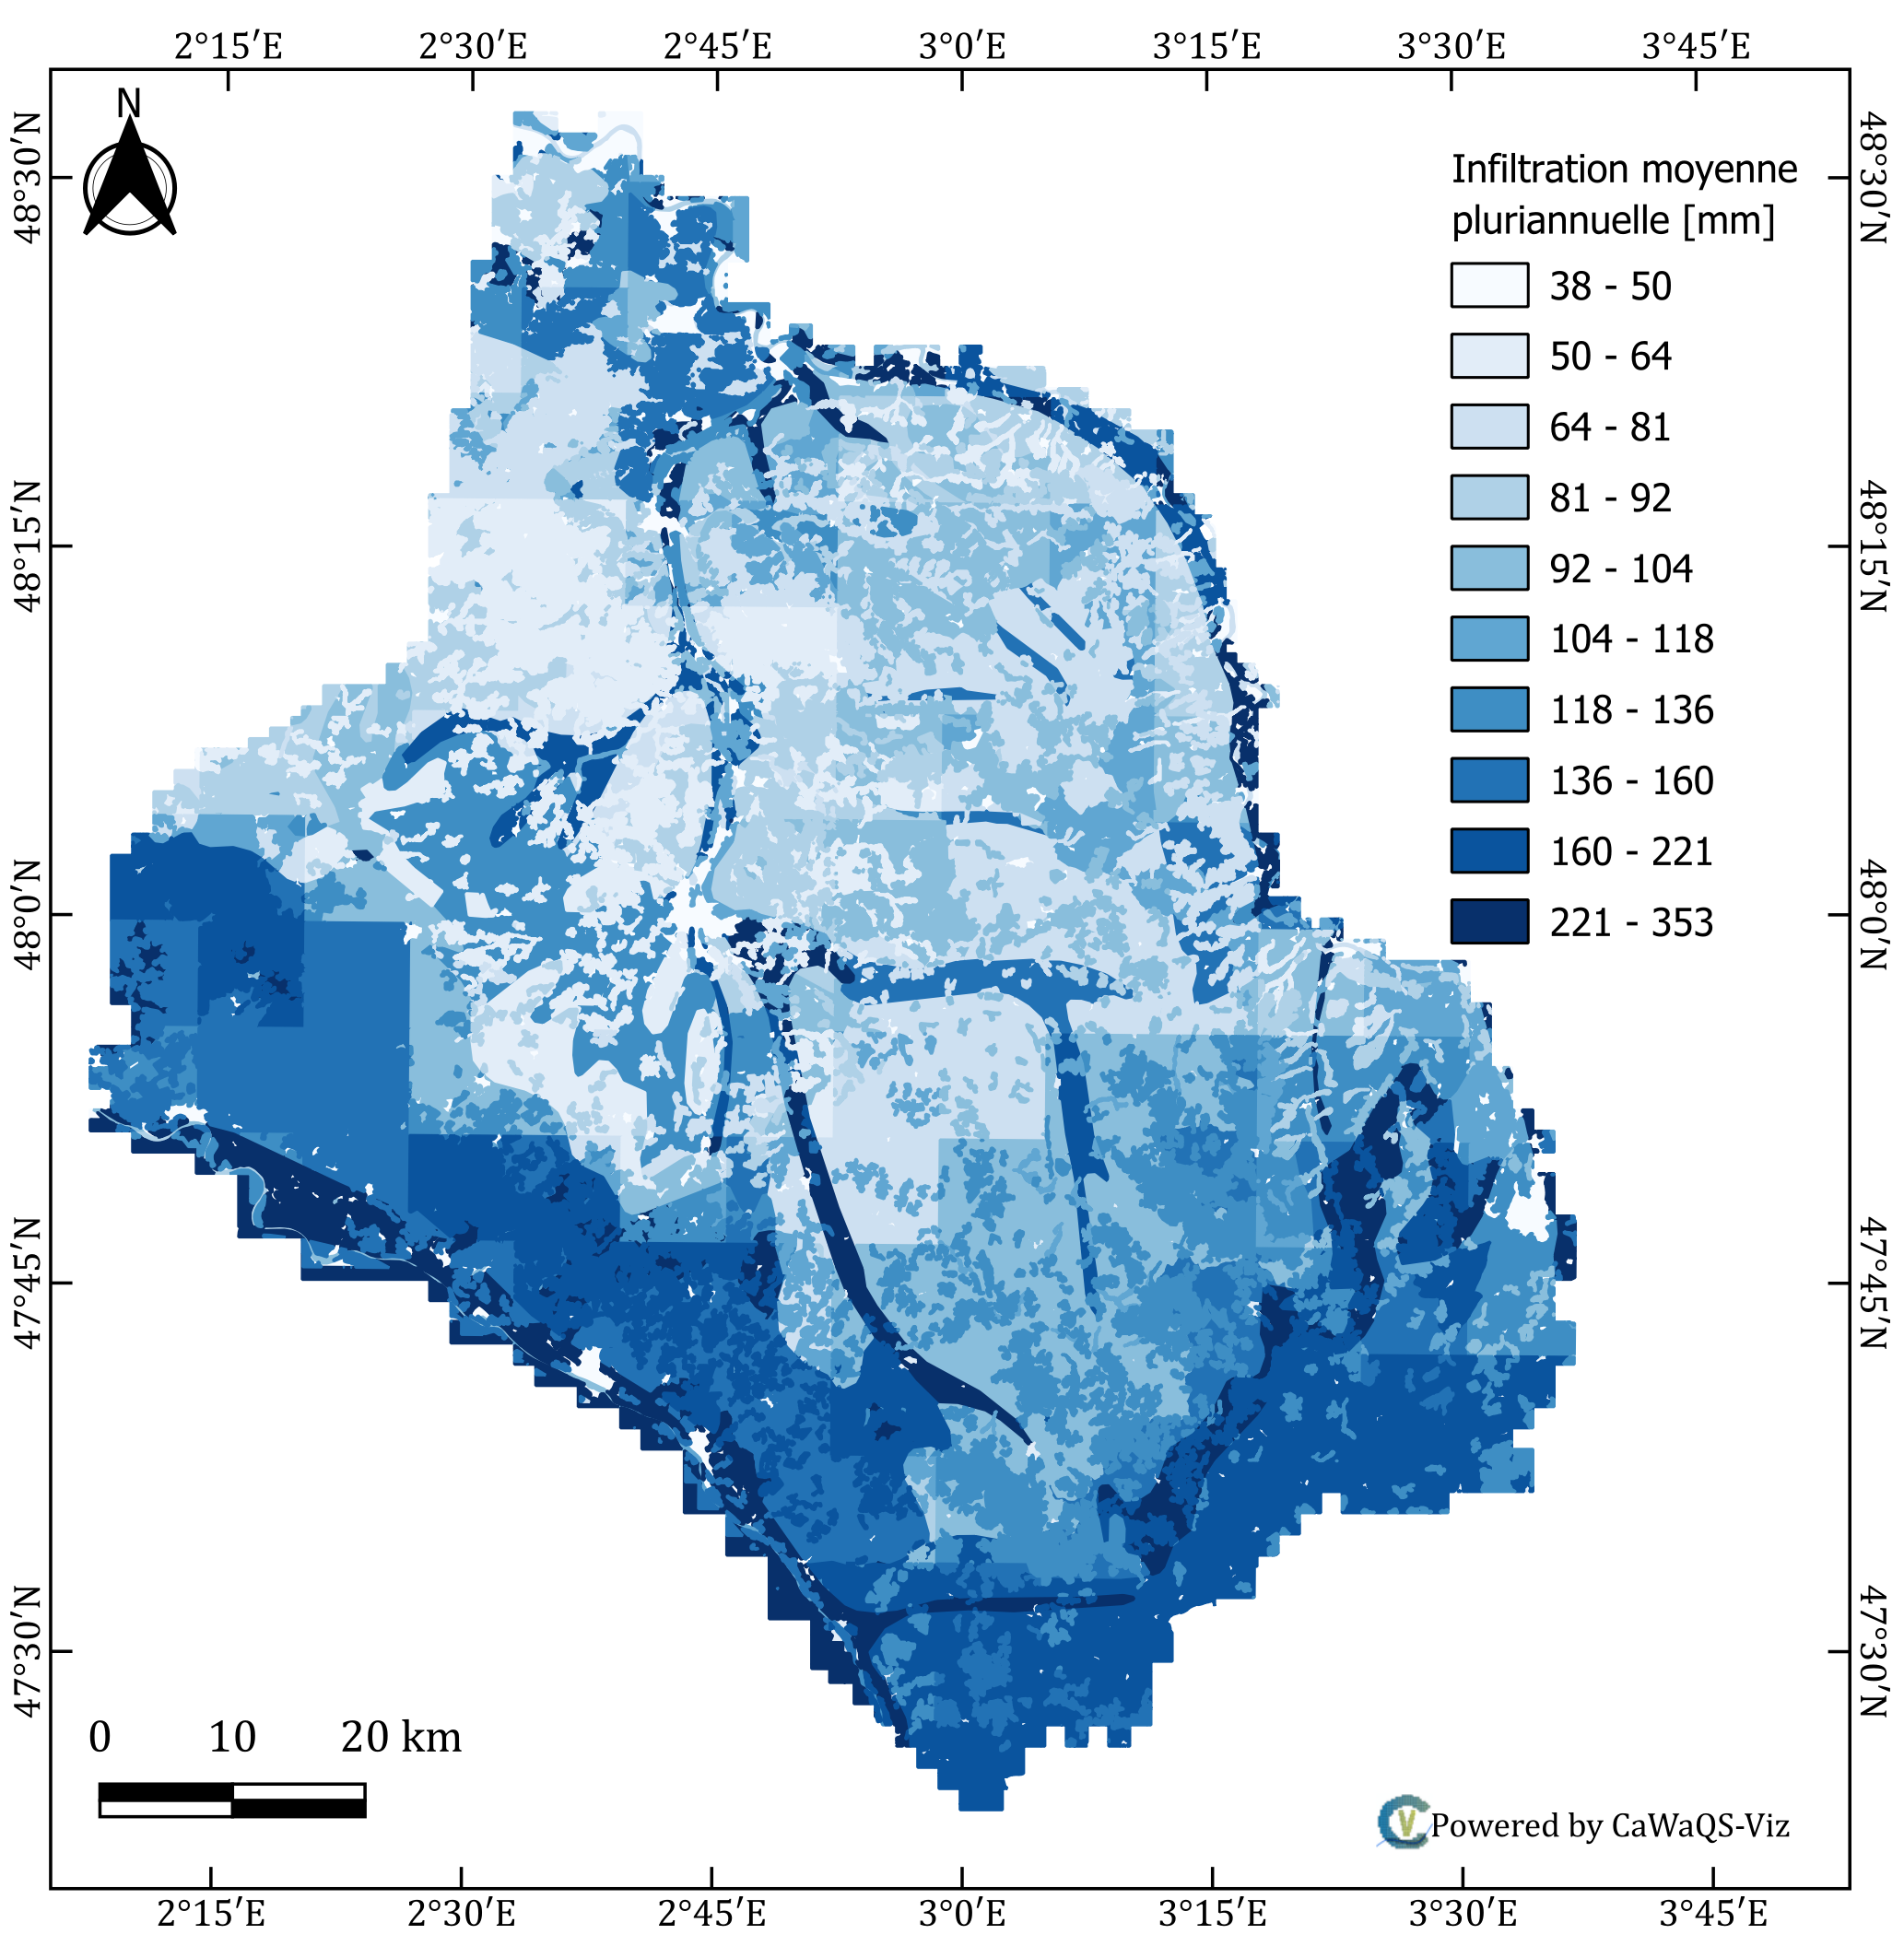
\includegraphics[width=\linewidth]{3_features/fig/OutputSpatialMap.png}
        \caption{}
        \label{fig-outSpatialMap-surf}
    \end{subfigure}
    \begin{subfigure}
        [b]{0.45\linewidth}
        \centering
        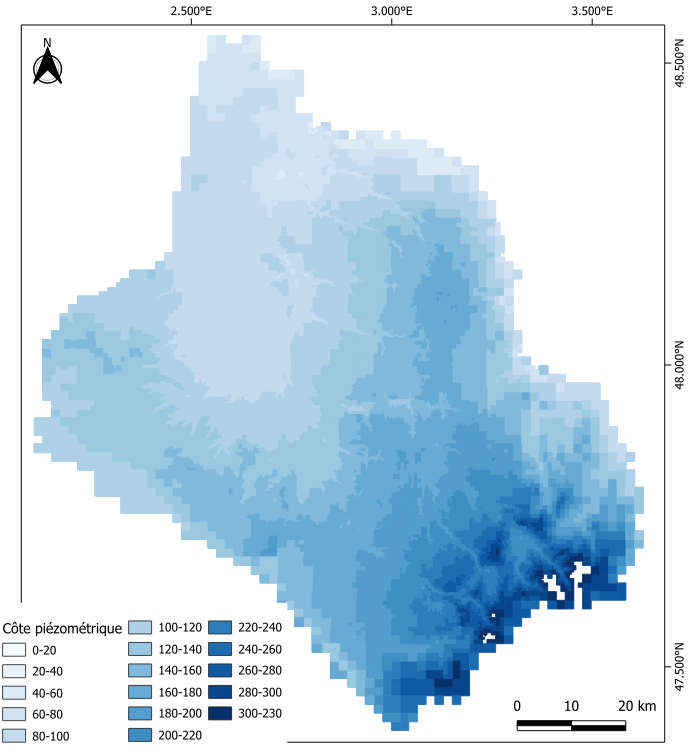
\includegraphics[width=\linewidth]{3_features/fig/Cote_piezo.png}
        \caption{}
        \label{fig-outSpatialMap-sout}
    \end{subfigure}
    \caption{Spatialisation du flux d'infiltration moyen interannuel [$mm$] (a)
    et de la piézométrie [$mNGF$] (b) simulé à l'échelle de l'hydrosystème du
    Loing }
    \label{fig:two_figures}
\end{figure}

Les valeurs prises par la variable hydrologique à spatialiser sont contenues dans
la table attributaire de la résolution \script{.shp} de sortie. La table a pour
colonnes les identifiants des années pour une agrégation annuelle, les identifiants des
mois pour une agrégation mensuelle et enfin la date pour une sortie des variables
à pas de temps journalier. Une agrégation pluriannuelle moyenne est également
possible en cochant la case \script{Pluriannual}, établissant ainsi un bilan
pluriannuel ou mensuel pluriannuel.

\begin{itemize}
    \item \script{WATBAL} : les variables de précipitations, ETR, ruissellement
        et infiltration (\ref{fig-outSpatialMap-surf}) ;

    \item \script{AQ} : les charges hydrauliques (\ref{fig-outSpatialMap-sout}), visualisables soit sur une couche
        du maillage aquifère donnée, soit sur les mailles aquifères à l'affleurement
        (maillage unique, créé par \cwv).\\
\end{itemize}

Les variables du compartiment \script{WATBAL} sont exprimées en \mmj~ou \mman~selon
le mode d'agrégation choisi. Les variables du compartiment \script{AQ} sont exprimées
en mètres.

\section{\script{Budget Bar Plot}: Visualisation du bilan hydrologique}
\label{sec-bufget-barplot}

Les bilans hydrologiques simulés peuvent être visualisés depuis cette boite de
dialogue. Ils sont construits en cohérence avec la période renseignée. Le champ
\script{Frequences} renseigne le pas de calcul du bilan hydrique (pluriannuel, annuel,
mensuel ou journalier), tandis que \script{agregator} renseigne l'agrégateur temporelle
(moyen, somme, maximum, minimum). Le bilan hydrique est aggrégé spatialement par
une moyenne des variables hydrologiques sur l'ensemble des mailles de surface.

À l'exécution de cette boîte de dialogue, une page \script{HTML} s'ouvre dans votre
navigateur et affiche un graphique interactif du bilan d'hydrologique. Une image
statique (cf. Fig. \ref{fig-budget-barplot}) de ce même graphique est
enregistrée dans le répertoire de post-process dans un sous-dossier \script{../BUDGET}
du répertoire de post-traitement.

\begin{figure*}[htb]
    \centering
    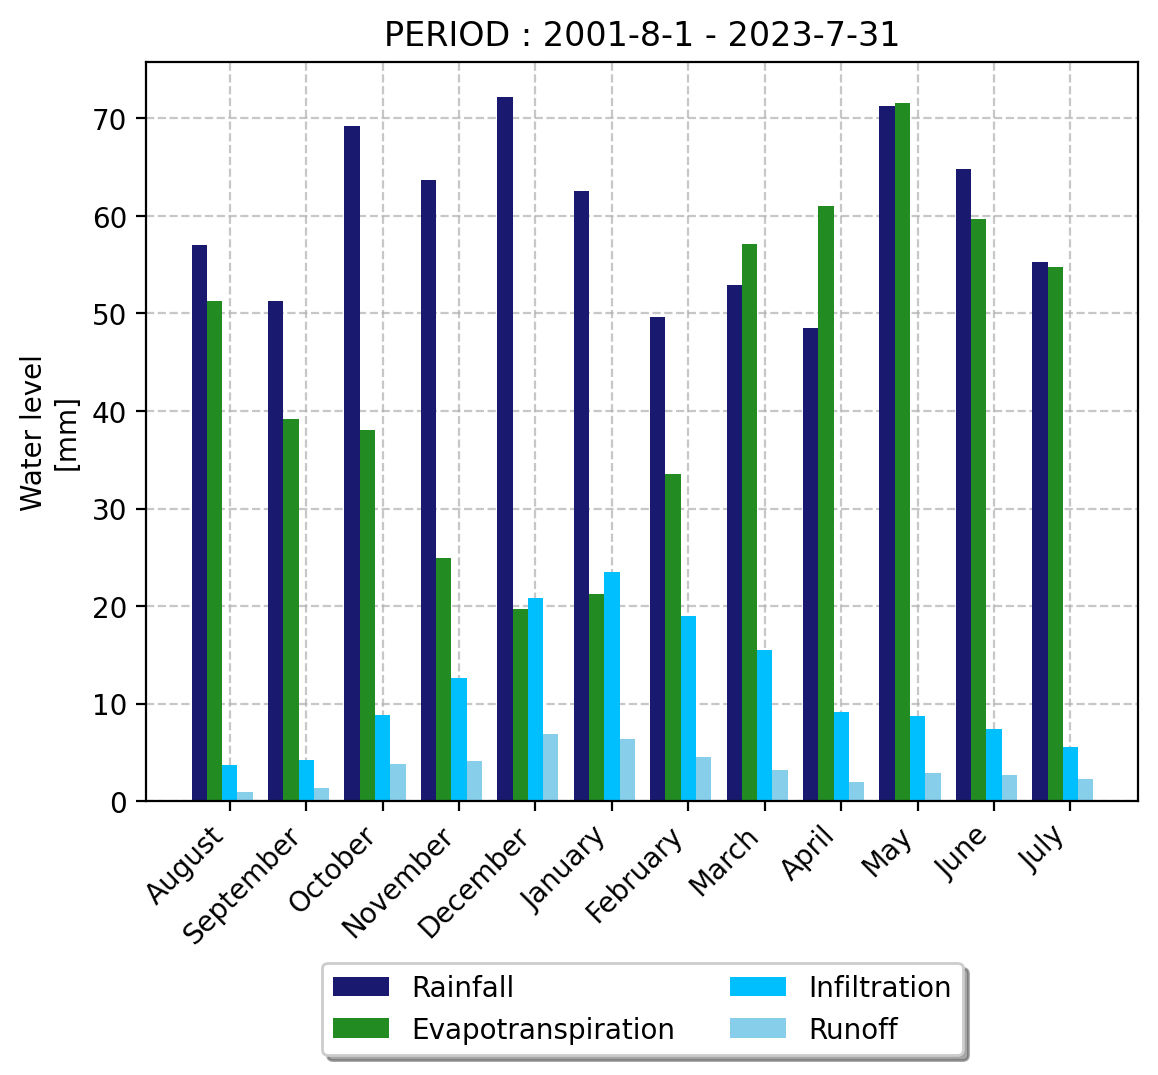
\includegraphics[width=0.55\linewidth]{
        3_features/fig/BUDGET_2001-8-12023-7-31Pluriannual_Sum.png
    }
    \caption{Exemple de rendu graphique du bilan hydrologique mensuel
    pluriannuel simulé}
    \label{fig-budget-barplot}
\end{figure*}

\newpage
\section{\script{Hydological Regime}: Visualisation des régimes hydrologiques}
\label{sec-regime-hydro}

Les régimes hydrologiques de l'hydrosystème simulés sont construits à partir de la
boite de dialogue \gui{Hydrological Regime} (cf. Figure
\ref{fig-dialogHydroRegime}). Les régimes hydrologiques sont calculés sur la
période renseignée dans les zones de saisie \gui{Start} et \gui{end}. La variable
analysée est à préciser dans le menu déroulant \gui{Hydrological variable to plot}. Le type de rendu est choisi par l'utilisateur en cochant les case \gui{static plots (PNG)} pour un rendu des graphiques sous la forme d'image unique pour chaque point de mesure, \gui{static plots (PDF)} pour un rendu sous forme pdf compilant les régimes hydrologiques de tous les points de mesure et enfin \gui{interractives plots} pour un rendu dans le navigateur par défaut sous la forme de graphique interactifs (\ref{fig-output-regime-hydrologique}. Une boite de dialogue avertit l'utilisateur de la fin de l'exécution du module de calcul.\\

\begin{figure}[h]
    \centering
    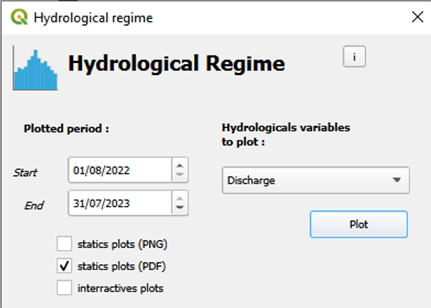
\includegraphics[width=0.5\linewidth]{
        3_features/fig/DialogHydrologicalREgime.png
    }
    \caption{Boite de dialogue \gui{Hydrological Regime} permettant le calcul des
    régimes hydrologiques mensuels pluriannuels.}
    \label{fig-dialogHydroRegime}
\end{figure}


\begin{figure*}[htb]
    \centering
    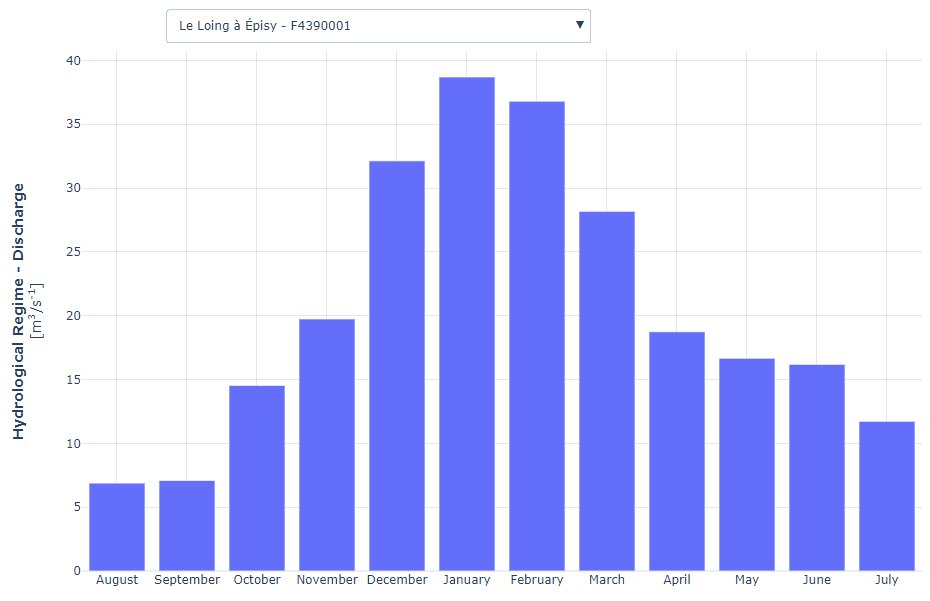
\includegraphics[width=0.5\linewidth]{
        3_features/fig/Output_regime_hydrologique.png
    }
    \caption{Exemple de rendu graphique du régime hydrologique mensuel
    pluriannuel simulé}
    \label{fig-output-regime-hydrologique}
\end{figure*}

\newpage
\section{\script{Extract Data from a sub area}: Extraction des resultats dans un polygon}
\label{sec-extract-area}

La boîte de dialogue \gui{Extract Data from a Sub Area} permet d’extraire les résultats des simulations sur une zone définie. Cette zone peut être spécifiée soit comme un polygone provenant d’un QGSVectorLayer chargé dans le projet, soit comme un shapefile importé depuis un répertoire.

Les résultats sont enregistrés sous forme de fichiers CSV (analyses) et de fichiers NumPy contenant les données de la zone extraite. Ces fichiers permettent de relancer les analyses à partir de la configuration créée.

\subsection*{Variables d’extraction}
À partir de la boîte de dialogue, il est possible de choisir les variables suivantes pour l’extraction :
\begin{itemize}
    \item Nom du nouveau fichier d’extraction (également utilisé comme nom du dossier créé dans \texttt{PostProcessing/DATA\_EXTRACTED/})
    \item Polygone d’extraction : soit un shapefile (à tester), soit un QGSVectorLayer présent dans le projet
    \item Période d’extraction
    \item Résolution de l’extraction pour le module WATBAL (à confirmer si nécessaire)
\end{itemize}

Les sorties dépendent des cases cochées dans la colonne de droite.

\subsection*{Sorties -- Bilan hydrologique (WATBAL)}
\gui{Rainfall} \gui{Real EvapoTranspiration (ET)} \gui{Infiltration} \gui{Runoff} \gui{Potential EvapoTranspiration (ET)}

Ces options fournissent les résultats du bilan hydrologique (WATBAL). Les données sont sauvegardées dans un fichier CSV sous forme agrégée sur toute la période de simulation, avec une valeur par cellule.

\subsection*{Sorties -- Régime hydrologique (HYD)}
\gui{Surface flow}

\begin{itemize}
    \item Tous les biefs en contact avec la bordure du polygone sont définis comme points d’extraction.
    \item Le fichier CSV contient les données journalières de débit et de hauteur d’eau pour chaque point situé sur la limite du polygone.
    \item La convention de signe pour le débit est la suivante : positif en entrée, négatif en sortie.
    \item Des fichiers NumPy sont également générés, permettant de relancer et d’approfondir les analyses sur ces données.
\end{itemize}

\subsection*{Sorties -- Aquifère}
\gui{Subsurface flow}

\begin{itemize}
    \item Pour chaque couche de l’aquifère, les limites du polygone sont définies avec la résolution propre à la couche.
    \item Un fichier CSV est généré pour chaque couche.
    \item Les flux sont fournis à une échelle journalière pour chaque face située à la limite de l’aquifère.
    \item Les faces sont nommées selon la convention : \texttt{nCell(ID\_ABS)\_direction\_unité}, par exemple : \texttt{3323\_west\_m3d}.
\end{itemize}

\subsection*{Organisation des outputs}

Pour chaque extraction, des fichiers de résultats et des couches sont produits.

Les fichiers sont sauvegardés dans le répertoire de sortie défini dans les paramètres de l’analyse principale :
\texttt{PostProcessing/DATA\_EXTRACTED/<Nom\_Extraction>}

On y trouve :
\begin{itemize}
    \item \textbf{CONFIG/} : fichiers de configuration permettant de relancer les simulations
    \item \textbf{OUTPUT/} : fichiers CSV contenant les résultats
    \item \textbf{TEMP/} : fichiers NumPy utilisés pour relancer les analyses
\end{itemize}

Dans QGIS, des maillages (\textit{mesh}) sont également générés pour chaque compartiment extrait.